\model{Static Variables}

Consider the definition for a bank account:

\medskip
\begin{javalst}
public class BankAccount {
    private static final String PREFIX = "1234";
    private static int nextNumber = 1;

    private String number;
    private String owner;
    private double balance;

    public BankAccount(String owner) {
        this.number = PREFIX + String.format("%04d", nextNumber);
        this.owner = owner;
        nextNumber++;
    }
}
\end{javalst}

\bigskip
Here is a memory diagram of two \java{BankAccount} objects:

\begin{javalst}
public static void main(String[] args) {
    BankAccount ba1 = new BankAccount("Stacie");
    BankAccount ba2 = new BankAccount("Trevor");
}
\end{javalst}

\hfill 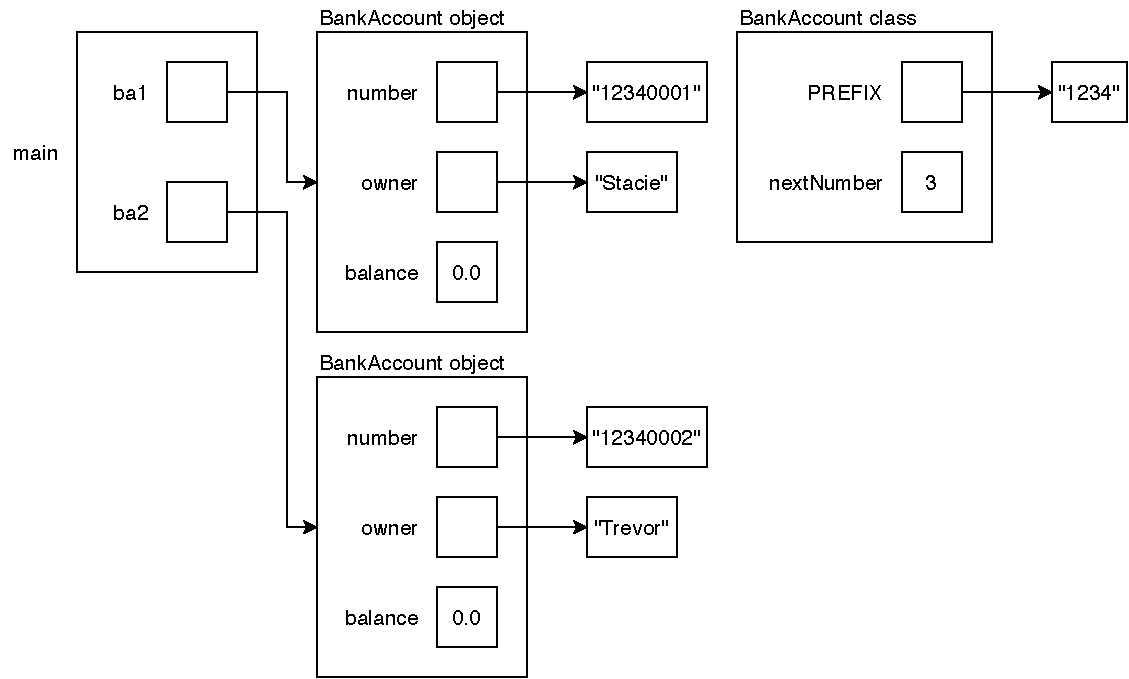
\includegraphics[width=\linewidth]{diagram-static.pdf}
\hspace{2em} \null


\quest{15 min}


\Q Based on the source code and memory diagram:

\begin{enumerate}
\item How many \java{BankAccount} variables were declared? \ans[3em]{2}
\item How many \java{BankAccount} objects were created? \ans[3em]{2}
\end{enumerate}


\Q How many instances of each variable are in memory?

\begin{multicols}{2}
\begin{enumerate}
\item \java{PREFIX} \ans[3em]{1}
\item \java{nextNumber} \ans[3em]{1}
\item \java{number} \ans[3em]{2}
\item \java{owner} \ans[3em]{2}
\item \java{balance} \ans[3em]{2}
\end{enumerate}
\end{multicols}


\Q \label{key3}
What is the difference between \java{static} and non-\java{static} variables of a class?
Explain your answer in terms of the diagram.

\begin{answer}[5em]
Static variables are shared by all instances of the class.
They are shown in the box labeled ``BankAccount class''.
Non-static variables are specific to each object.
They are shown in boxes labeled ``BankAccount object''.
\end{answer}


\Q Why are all the strings shown in separate boxes as opposed to being written inside of the variable boxes?

\begin{answer}
Strings are objects, so their variables contain references.
(There is not enough memory inside the variable to store the entire string.)
\end{answer}


\Q How would you modify the memory diagram if the following line were added at the end of the \java{main} method?

\begin{javalst}
BankAccount ba3 = ba2;
\end{javalst}

\begin{answer}
Add a new box for \java{ba3} and draw an arrow to the object for \java{ba2}.
Notice that assigning reference types does not create new objects!
\end{answer}


\Q (Optional) Paste the contents of \textit{BankAccount.java} into \href{https://cscircles.cemc.uwaterloo.ca/java_visualize/#code=public+class+ClassNameHere+%7B%0A++++public+static+void+main(String%5B%5D+args)+%7B%0A++++++++%0A++++%7D%0A%7D&mode=edit&showStringsAsObjects=1}{Java Visualizer}.
What differences do you notice between the diagram in Java Visualizer and those in \ref{\currfilename}?

\begin{answer}
Answers might include:
\bull The static fields are drawn above the top frame.
\bull The strings are drawn inside the objects (for convenience).
\end{answer}
